% Kurze Lesefassung; kanonische Aussagen und Tabellen stehen in Band 19.
\section*{Mit diesem Heft arbeiten}
\addcontentsline{toc}{section}{Mit diesem Heft arbeiten}

Eine Zahl lässt sich durch alles beschreiben, was unter ihr liegt.
Dedekindsche Schnitte machen aus diesem Gedanken eine Konstruktion:
Aus rationalen Zahlen entsteht eine vollständig geordnete Menge.
Ihr entscheidender Satz passt in eine Zeile:
\[
 \boxed{\sup\mathcal A=\bigcup\mathcal A.}
\]
Die Voraussetzungen und der Beweis dieser Formel sind das Ziel des Hefts.

\textbf{Voraussetzungen.}
Wir verwenden die rationalen Zahlen $\mathbb Q$, ihre Rechenregeln
und ihre Ordnung sowie Teilmengen, Vereinigung und Funktionen.
Zwischen $p<q$ liegt die rationale Zahl $(p+q)/2$.
Folgen, Grenzwerte und reelle Rechenoperationen werden nicht vorausgesetzt.

\textbf{Lesen und ausprobieren.}
Die rechte Karoseite gehört jeweils zum Text links. Halte dort einen
Beweis in eigenen Worten fest oder zeichne ein Beispiel.
Das separate \href{_B19-cuts-exercises.pdf\#cuts.exercises}{Übungsheft} bietet acht Aufgaben und vollständige Lösungen.

\textbf{Dein Lesepfad.}
\begin{center}
\renewcommand{\arraystretch}{1.16}
\begin{tabularx}{\linewidth}{@{}Xr@{}}
\toprule
Thema & ab Seite\\
\midrule
\hyperref[cuts:idea]{Schnittidee und Hauptschnitte} & \pageref{cuts:idea}\\
\hyperref[cuts:order]{Ordnung und rationale Einbettung} & \pageref{cuts:order}\\
\hyperref[cuts:supremum]{Vereinigung und Vollständigkeit} & \pageref{cuts:supremum}\\
\hyperref[cuts:example]{Ein Beispiel und die Voraussetzungen} & \pageref{cuts:example}\\
\hyperref[cuts:correspondence]{Zuordnung zu den Beweistabellen} & \pageref{cuts:correspondence}\\
\hyperref[cuts:history]{Historischer Abriss und Schlussbemerkung} & \pageref{cuts:history}\\
\bottomrule
\end{tabularx}
\end{center}

\clearpage
\section{Eine Zahl von unten beschreiben}
\label{cuts:idea}

Was wissen wir über die rationale Zahl $1$, wenn wir nur wissen,
welche rationalen Zahlen kleiner als $1$ sind?
Wir kennen die Menge
\[
 \widehat 1=\{p\in\mathbb Q:p<1\}.
\]
Sie enthält beispielsweise $-2$, $0$ und $3/4$, aber weder $1$ noch $5/4$.
Ein einzelner Eintrag verrät wenig. Die ganze Menge beschreibt die
Position der $1$ eindeutig.

\begin{center}
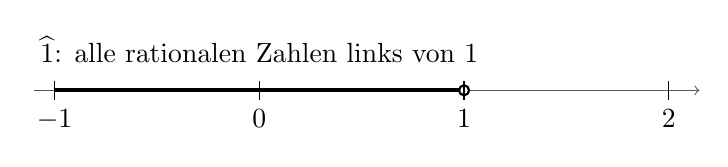
\begin{tikzpicture}[x=26mm,y=9mm]
 \draw[->,black!65] (-1.1,0)--(2.15,0);
 \draw[line width=1.5pt] (-1,0)--(1,0);
 \draw[fill=white,line width=.8pt] (1,0) circle (1.8pt);
 \foreach \x/\lab in {-1/{-1},0/{0},1/{1},2/{2}} {
  \draw (\x,-.13)--(\x,.13);
  \node[below] at (\x,-.13) {$\lab$};
 }
 \node[above] at (0,.25) {$\widehat1$: alle rationalen Zahlen links von $1$};
\end{tikzpicture}
\end{center}
Die Skizze zeigt die Lage; die Menge besteht nur aus rationalen Zahlen.
Der offene Kreis erinnert daran, dass die Randzahl nicht dazugehört.

Für jede rationale Zahl $q$ können wir ebenso $\widehat q$ bilden.
Der nächste Schritt ist entscheidend: Wir beschreiben passende Mengen
\emph{durch ihre Eigenschaften}, ohne vorher eine Randzahl zu verlangen.
Solche Mengen werden selbst unsere neuen Zahlen.

\textbf{Die Leitfrage.}
Welche Eigenschaften muss ein rationaler Anfangsabschnitt besitzen,
damit er eine Zahl darstellen kann?

\clearpage
\section{Vier Bedingungen für einen Schnitt}
\label{cuts:definition}

\begin{definition}
Eine Teilmenge $A\subseteq\mathbb Q$ heißt \emph{Dedekindscher Schnitt},
wenn folgende vier Bedingungen gelten:
\begin{enumerate}
 \item $A$ ist nicht leer.
 \item $A$ ist nicht ganz $\mathbb Q$.
 \item Mit $p\in A$ gehört jede rationale Zahl $q<p$ zu $A$.
 \item Zu jedem $p\in A$ gibt es ein $r\in A$ mit $p<r$.
\end{enumerate}
\end{definition}
Die dritte Bedingung heißt \emph{nach unten abgeschlossen};
die vierte sagt: $A$ hat kein größtes Element.

Die ersten beiden Bedingungen halten den Schnitt von beiden Enden fern:
Es gibt eine rationale Zahl darin und eine außerhalb.
Die dritte verbietet Löcher unterhalb eines enthaltenen Elements.
Die vierte legt fest, wie wir mit einem rationalen Rand umgehen.

\begin{beispiel}
Die Menge $\{p\in\mathbb Q:p\leq1\}$ hat das größte Element $1$.
Sie ist deshalb kein Schnitt. Die Menge $\widehat1$ erfüllt dagegen
alle vier Bedingungen. Für $p<1$ liegt $(p+1)/2$ noch näher an $1$
und weiterhin unter $1$.
\end{beispiel}

\textbf{Warum die Randbedingung?}
Ohne sie würden sowohl $\{p:p<1\}$ als auch $\{p:p\leq1\}$
dieselbe vertraute Randlage beschreiben. Wir entscheiden uns einheitlich
für Anfangsabschnitte ohne größtes Element.

\clearpage
\section{Die rationalen Hauptschnitte}
\label{cuts:principal}

\begin{definition}
Für $q\in\mathbb Q$ heißt
\[
 \widehat q=\{p\in\mathbb Q:p<q\}
\]
der \emph{Hauptschnitt} von $q$.
\end{definition}

\begin{satz}
Jeder rationale Hauptschnitt ist ein Dedekindscher Schnitt.
\end{satz}
\begin{proof}
$q-1$ gehört zu $\widehat q$, $q$ selbst nicht.
Damit ist $\widehat q$ weder leer noch ganz $\mathbb Q$.
Aus $s<p<q$ folgt $s<q$: Der Schnitt ist nach unten abgeschlossen.
Schließlich gilt für jedes $p<q$
\[
 p<\frac{p+q}{2}<q.
\]
Also gibt es kein größtes Element.
\end{proof}

Der Beweis prüft genau die vier Bedingungen. Die letzte Prüfung benutzt
die Dichte der rationalen Ordnung: Zwischen zwei verschiedenen rationalen
Zahlen ist immer noch Platz.

\begin{beispiel}
In $\widehat{3/2}$ liegen $1$, $7/5$ und $149/100$.
Keine dieser Zahlen ist die größte. Die Zahl $3/2$ beschreibt den Rand,
gehört aber selbst nicht zur Menge.
\end{beispiel}

\textbf{Zwei verschiedene Dinge.}
$q$ ist eine rationale Zahl; $\widehat q$ ist eine Menge rationaler Zahlen.
Die Konstruktion verbindet beide, ohne sie vorzeitig gleichzusetzen.

\clearpage
\section{Die neuen Zahlen und ihre Ordnung}
\label{cuts:order}

Wir sammeln sämtliche Schnitte in einer Menge:
\[
 \mathbb R=\{A\subseteq\mathbb Q:A\text{ ist ein Schnitt}\}.
\]
Das ist eine Teilmenge der Potenzmenge von $\mathbb Q$.
In diesem Modell ist eine reelle Zahl also selbst ein Schnitt.

Ein weiter rechts liegender Rand hat mehr rationale Zahlen unter sich.
Das legt die Ordnung fest:
\begin{definition}
Für $A,B\in\mathbb R$ setzen wir
\[
 A\leq_{\mathbb R}B\quad\Longleftrightarrow\quad A\subseteq B,
 \qquad
 A<_{\mathbb R}B\quad\Longleftrightarrow\quad A\subsetneq B.
\]
\end{definition}

Drei Ordnungsgesetze erhalten wir unmittelbar von der Inklusion:
\begin{itemize}
 \item $A\subseteq A$: Jede Zahl ist mit sich selbst vergleichbar.
 \item Aus $A\subseteq B$ und $B\subseteq A$ folgt $A=B$.
 \item Aus $A\subseteq B\subseteq C$ folgt $A\subseteq C$.
\end{itemize}
Das sind Reflexivität, Antisymmetrie und Transitivität.

Bei beliebigen Teilmengen reicht dies noch nicht für eine totale Ordnung.
Zum Beispiel enthält weder $\{0\}$ die Menge $\{1\}$ noch umgekehrt.
Für Schnitte gelingt der Vergleich immer. Dafür sorgt ihr
Abschluss nach unten.

\clearpage
\section{Warum zwei Schnitte immer vergleichbar sind}
\label{cuts:total}

\begin{satz}
Für Schnitte $A,B$ gilt stets $A\subseteq B$ oder $B\subseteq A$.
Die Inklusion ist auf $\mathbb R$ daher eine totale Ordnung.
\end{satz}

\Beweisidee Wenn $A$ über $B$ hinausragt, liegt bereits ganz $B$ unter
einem einzigen Element von $A$.

\begin{proof}
Falls $A\subseteq B$ gilt, sind wir fertig. Andernfalls wähle
$p\in A\setminus B$. Jedes $b\in B$ erfüllt $b<p$:
Bei $b=p$ wäre $p\in B$; bei $p<b$ würde der Abschluss von $B$
nach unten ebenfalls $p\in B$ ergeben.
Weil $p\in A$ und $b<p$, gehört jedes $b\in B$ zu $A$.
Somit ist $B\subseteq A$.
\end{proof}

\begin{center}
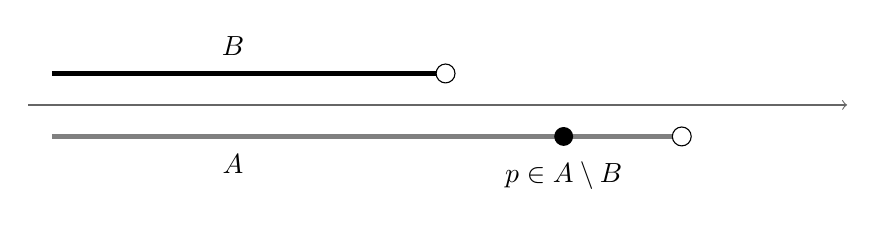
\begin{tikzpicture}[x=1mm,y=1mm]
 \draw[->,black!60] (0,0)--(104,0);
 \draw[line width=1.6pt] (3,4)--(53,4);
 \draw[line width=1.6pt,black!50] (3,-4)--(83,-4);
 \draw[fill=white] (53,4) circle (1.2mm);
 \draw[fill=white] (83,-4) circle (1.2mm);
 \fill (68,-4) circle (1.2mm);
 \node[above] at (26,5) {$B$};
 \node[below] at (26,-5) {$A$};
 \node[below] at (68,-6) {$p\in A\setminus B$};
\end{tikzpicture}
\end{center}
Die Skizze stellt den zweiten Fall dar. Im Beweis brauchen wir keinen
vorhandenen Randpunkt. Der rationale Zeuge $p$ genügt.

\textbf{Merksatz.}
Anfangsabschnitte einer totalen Ordnung sind ineinander geschachtelt.

\clearpage
\section{Die alte Ordnung bleibt erhalten}
\label{cuts:embedding}

Die Abbildung $\iota:\mathbb Q\to\mathbb R$, $q\mapsto\widehat q$,
setzt jede rationale Zahl an ihren Platz im neuen Modell.

\begin{satz}
Für $p,q\in\mathbb Q$ gilt
\[
 p\leq q\quad\Longleftrightarrow\quad\widehat p\subseteq\widehat q.
\]
Außerdem gilt $p<q$ genau dann, wenn
$\widehat p\subsetneq\widehat q$. Insbesondere ist $\iota$ injektiv.
\end{satz}

\begin{proof}
Ist $p\leq q$, so folgt aus $x<p$ auch $x<q$.
Also ist $\widehat p\subseteq\widehat q$.
Gilt umgekehrt diese Inklusion, kann nicht $q<p$ sein:
Dann läge $q$ in $\widehat p$, aber nicht in $\widehat q$.
Somit ist $p\leq q$.

Bei $p<q$ gehört $p$ zu $\widehat q\setminus\widehat p$;
die Inklusion ist also echt. Eine echte Inklusion liefert nach der
ersten Aussage $p\leq q$ und schließt $p=q$ aus.
Aus $\widehat p=\widehat q$ folgen schließlich $p\leq q$ und $q\leq p$,
also $p=q$.
\end{proof}

\begin{beispiel}
Aus $0<1/2<1$ wird
\[
 \widehat0\subsetneq\widehat{1/2}\subsetneq\widehat1.
\]
Die rationalen Zahlen werden weder vertauscht noch miteinander verschmolzen.
Ihre Bilder bilden eine ordnungstreue Kopie in $\mathbb R$.
\end{beispiel}

\clearpage
\section{Was Vollständigkeit verlangt}
\label{cuts:supremum}

Jetzt geht es um eine \emph{Familie von Schnitten} $\mathcal A\subseteq\mathbb R$.
Ihre Mitglieder sind reelle Zahlen des neuen Modells.

\begin{definition}
Ein Schnitt $U$ heißt \emph{obere Schranke} von $\mathcal A$, wenn
\[
 A\subseteq U\qquad\text{für jedes }A\in\mathcal A.
\]
Ein Schnitt $S$ heißt \emph{Supremum} von $\mathcal A$, wenn er
obere Schranke ist und in jeder oberen Schranke enthalten ist.
Wir schreiben $S=\sup\mathcal A$.
\end{definition}
Ein Supremum ist damit die kleinste obere Schranke.
Es muss nicht zur Familie gehören. Gehört es dazu, ist es zugleich
ihr größtes Mitglied, also ihr \emph{Maximum}.

\textbf{Unser Ziel.}
Jede nichtleere, nach oben beschränkte Familie von Schnitten
soll ein Supremum besitzen. Diese Eigenschaft heißt hier
\emph{Vollständigkeit der Ordnung}.

\begin{beispiel}
Für $\mathcal A=\{\widehat0,\widehat{1/2}\}$ ist $\widehat1$
eine obere Schranke. Die kleinste ist $\widehat{1/2}$.
Hier ist das Supremum auch ein Maximum.
\end{beispiel}

\textbf{Die Idee für beliebige Familien.}
Eine obere Schranke muss alles enthalten, was in irgendeinem Mitglied
vorkommt. Wir sammeln deshalb genau diese rationalen Zahlen.

\clearpage
\section{Alle unteren Zahlen einsammeln}
\label{cuts:union-cut}

Sei $\varnothing\ne\mathcal A\subseteq\mathbb R$, und sei $U\in\mathbb R$
eine obere Schranke. Wir bilden
\[
 S=\bigcup\mathcal A
  =\{p:\text{für ein }A\in\mathcal A\text{ gilt }p\in A\}.
\]
Zunächst müssen wir prüfen, ob $S$ überhaupt eine reelle Zahl ist.

\begin{satz}
Die Vereinigung $S$ ist ein Dedekindscher Schnitt.
\end{satz}
\begin{proof}
Alle Mitglieder sind Teilmengen von $\mathbb Q$, also auch $S$.
Wähle ein $A_0\in\mathcal A$. Weil $A_0$ nicht leer ist und $A_0\subseteq S$ gilt,
ist $S$ nicht leer.

Jedes $A\in\mathcal A$ liegt in $U$. Daher ist $S\subseteq U$.
Weil $U\ne\mathbb Q$, gilt auch $S\ne\mathbb Q$.

Sei nun $p\in S$. Dann liegt $p$ in einem Mitglied $A\in\mathcal A$.
Jede rationale Zahl $q<p$ gehört schon zu diesem $A$, also zu $S$.
Außerdem enthält dieses $A$ ein $r>p$. Somit besitzt auch $S$
kein größtes Element.
\end{proof}

\textbf{So verteilt sich die Arbeit.}
Die Nichtleerheit der Familie liefert einen Anfang.
Die obere Schranke verhindert, dass wir ganz $\mathbb Q$ einsammeln.
Die beiden übrigen Schnittbedingungen erbt $S$ jeweils von einem
passenden Mitglied der Familie.

\clearpage
\section{Die Vereinigung ist das Supremum}
\label{cuts:complete}

\begin{satz}[Vollständigkeit]
Jede nichtleere, nach oben beschränkte Familie
$\mathcal A\subseteq\mathbb R$ besitzt ein Supremum. Es ist
\[
 \boxed{\sup\mathcal A=\bigcup\mathcal A.}
\]
\end{satz}

\begin{proof}
Nach Abschnitt~\ref{cuts:union-cut} ist $S=\bigcup\mathcal A$ ein Schnitt.
Jedes $A\in\mathcal A$ liegt in $S$; also ist $S$ eine obere Schranke.

Ist $V$ irgendeine obere Schranke, so liegt jedes $A\in\mathcal A$ in $V$.
Damit liegt auch ihre Vereinigung $S$ in $V$.
Also ist $S$ die kleinste obere Schranke.
\end{proof}

Die eigentliche Supremumseigenschaft ist damit sehr kurz bewiesen.
Die wesentliche Vorarbeit war die Frage, ob die Vereinigung noch
zum konstruierten Zahlbereich gehört.

\textbf{Warum ist das Supremum eindeutig?}
Sind $S$ und $T$ beide kleinste obere Schranken, so gilt
$S\subseteq T$ und $T\subseteq S$. Also ist $S=T$.
Deshalb dürfen wir von \emph{dem} Supremum sprechen.

\textbf{Zwei Ebenen, zwei Zeichen.}
In $p\in A$ ist $p$ eine rationale Zahl und $A$ ein Schnitt.
In $A\subseteq S$ sind $A$ und $S$ beide Schnitte.
Diese zweite Beziehung ist genau $A\leq_{\mathbb R}S$.

\clearpage
\section{Ein Supremum ohne größtes Mitglied}
\label{cuts:example}

Wir betrachten alle rationalen Hauptschnitte unterhalb von $\widehat1$:
\[
 \mathcal A=\{\widehat q:q\in\mathbb Q,\ q<1\}.
\]
Die Familie ist nicht leer, denn $\widehat0\in\mathcal A$.
$\widehat1$ ist eine obere Schranke.

\textbf{Welche Zahlen sammeln wir ein?}
Aus $p\in\widehat q$ und $q<1$ folgt $p<1$.
Also ist $\bigcup\mathcal A\subseteq\widehat1$.
Umgekehrt liegt zu jedem $p<1$ die rationale Zahl
\[
 q=\frac{p+1}{2}
\]
zwischen $p$ und $1$. Damit ist $\widehat q\in\mathcal A$ und
$p\in\widehat q$. Also gehört jedes $p\in\widehat1$ zur Vereinigung.
Zusammen ergibt das
\[
 \bigcup\mathcal A=\widehat1,
 \qquad \sup\mathcal A=\widehat1.
\]

\textbf{Warum gibt es kein Maximum?}
Zu jedem $q<1$ ist $r=(q+1)/2$ ebenfalls kleiner als $1$, aber größer als $q$.
Deshalb ist $\widehat q\subsetneq\widehat r$, und $\widehat r$ gehört
wieder zur Familie. Kein Mitglied ist das größte.

Das Supremum $\widehat1$ gehört selbst nicht zu $\mathcal A$.
Auch die rationale Zahl $1$ gehört nicht zum Schnitt $\widehat1$.
Das sind zwei verschiedene Aussagen auf den beiden Ebenen.

\clearpage
\section{Wozu die Voraussetzungen gebraucht werden}
\label{cuts:limits}

Der Vollständigkeitssatz verlangt eine \emph{nichtleere} und
\emph{nach oben beschränkte} Familie. Beide Bedingungen haben im Beweis
eine genaue Aufgabe.

\textbf{Eine leere Familie.}
Ihre Vereinigung ist $\varnothing$. Diese Menge ist kein Schnitt.
Die Formel $\sup\mathcal A=\bigcup\mathcal A$ liefert hier also
keine reelle Zahl. Über die leere Familie macht unser Satz keine Aussage.

\textbf{Eine unbeschränkte Familie.}
Nehmen wir alle rationalen Hauptschnitte:
\[
 \mathcal B=\{\widehat q:q\in\mathbb Q\}.
\]
Für jedes $p\in\mathbb Q$ gilt $p\in\widehat{p+1}$.
Daher ist $\bigcup\mathcal B=\mathbb Q$, ebenfalls kein Schnitt.
Eine obere Schranke $U\in\mathbb R$ müsste dann ganz $\mathbb Q$
enthalten. Das widerspräche der Echtheit von $U$.

\textbf{Die richtige Reihenfolge.}
Die Vereinigung einer Mengenfamilie ist immer eine Menge.
Um sie mit der \emph{reellen} Ordnung vergleichen zu dürfen,
müssen wir aber zuvor ihre Schnittbedingungen nachweisen.
Genau das leistet Abschnitt~\ref{cuts:union-cut}.

\textbf{Eine letzte Unterscheidung.}
Jeder einzelne Schnitt hat kein größtes rationales Element.
Eine Familie von Schnitten kann trotzdem ein größtes Mitglied haben,
wie das endliche Beispiel aus Abschnitt~\ref{cuts:supremum} zeigt.
